\documentclass[a4paper, 11pt]{article}

\usepackage[utf8]{inputenc} % UTF8 encoding
\usepackage[T1]{fontenc}
\usepackage{fullpage} % changes the margin
\usepackage[final]{pdfpages}
\usepackage{graphicx}
\usepackage{makecell}
\usepackage{listings}
\usepackage{varioref}
\usepackage{hyperref}
\usepackage{float}
\usepackage{amsmath}

% No idents
\setlength{\parindent}{0em}

\lstdefinestyle{customc++}{
  breaklines=true,
  xleftmargin=\parindent,
  language=C++,
  basicstyle=\footnotesize\ttfamily,
  keywordstyle=\bfseries\color{green!40!black},
  commentstyle=\itshape\color{purple!40!black},
  identifierstyle=\color{blue},
  stringstyle=\color{orange},
}

\lstset{style=customc++}

\begin{document}

\large\textbf{Ruprecht-Karls University of Heidelberg} \hfill \textbf{Teammates:} \\
\normalsize Institut für Theoretische Astrophysik \hfill 
H.Lüdemann (3589643), F.Wallberg (3548199), D.Wolf (3548138) \\
Prof. Dr. Ralf S. Klessen \hfill Exercise Date: 16/10/2019 \\
Tutor: Marcelo Barraza \hfill Due Date: 23/10/2019 \\


\section{Pitfalls of integer and floating point arithmetic}

The aim of the first exercise is to illustrate some pitfalls one can encounter when dealing
with in integer and floating point arithmetic in C and C++.\\
For this purpos some code samples are provided which should be executed and the results 
explained.

\subsection*{1. Sample}
The first code sample shows the difference between integer and floating point devision.
\begin{lstlisting}[language=C++]
    int   i = 7;
    float y = 2*(i/2);
    float z = 2*(i/2.);
    printf("%e %e \n", y,z); 
\end{lstlisting}
If executed this code returns the following numbers to the console 
for $x$ and $y$.

\begin{lstlisting}[language=C++]
    y = 6.000000e+00
    x = 7.000000e+00
\end{lstlisting}

Clearly the first number is wrong. The reason for this is that the calculation of 
$y$ is done as an integer devision. This devision cuts of the floating part of the number.
So the calculation $7/2$ gives the result 3. This is then multiplied by 2 and cast into a
floating point number. But if one of the numbers of the devision is marked as a floating 
point number like $7/2.$ then the correct result is calculated.

\subsection*{2. Sample}
\begin{lstlisting}[language=C++]
    double a = 1.0e17;
    double b = -1.0e15;
    double c = 1.0;
    double x = (a + b) + c;
    double y = a + (b + c);

\end{lstlisting}

If this second code sample is executed the following 
result is printed to the console for $x$ and $y$.

\begin{lstlisting}[language=C++]
    x = 1.000000e+00
    y = 0.000000e+00 
    
\end{lstlisting}

Again it is clear that only the result for $x$ is correct.
The problem with the second part is the summation of $b$
and $c$ which are numbers of very different magnitude.
When adding the numbers the small value will be converted
into a representation with the same exponent as the 
larg number. But the mantissa of the floating point number
can only cover a certain range and so the 1.0 will be represented
as a 0.0. \\
As a result the addition of the small and the large number 
returns the large number as a result and hence the final 
result is incorrect.
This problem does not occure if the two large numbers are 
substracted first.\\
So the reason why the law of associativity is broken in this
example is that computers can only add numbers with the same
exponent and that the mantissa of a floating point number
can only cover numbers in a certain range.\\


\subsection*{3. Sample}

\begin{lstlisting}[language=C++]
    float x = 1e20;
    float y;
    y = x * x;
    printf("%e %e\n", x,y/x);

\end{lstlisting}

The result of the last sample code is:
\begin{lstlisting}[language=C++]
    x = 1.000000e+20 
    y/x = 0.000000e+00
    
\end{lstlisting}

The problem in this case is that the maximum number that
can be represented with a float is approximately $3,4\textrm{e}38$
and therefore $y=1\textrm{e}40$ will actually be represented as infinity.
This is the reason why the devision $y/x$ gives as a result 0.0.\\
\section{Near-cancelation of numbers}

In this section the computation of the function

\begin{align}
    f(x) = \frac{x+e^{-x}-1}{x^2}
\end{align}

should be analysed.

\subsection{Calculating the lim.}

First the limit $\lim_{x\to 0}f(x)$ should be calculated. This can easily be done with L'Hôpital's rule.
\begin{align}
\lim_{x\to 0}\frac{x+e^{-x}-1}{x^2} = \lim_{x\to 0} \frac{1-e^{-x}}{2x} = \lim_{x\to 0}\frac{1+e^{-x}}{2}=\frac{1}{2}   
\end{align}


\subsection{Interactive program to compute the function.}

The interactive program for the computation of this function is lokated
in the file \textit{part2.cpp}. For easy compilation
a \textit{CMakeLists.txt} file is included to use with \textit{cmake}.
The different parts of the program can be used by specifying different command line 
arguments. For the interactive program choose 0 and for the evaluation of the 
function for small values choose 1 as a command line argument.


\subsection{Analyse critical small values.}

If the function is evaluated for small values the formula goes wrong.
To determine the value of x for which this happens, the function
is evaluated for a range of small values and the results are plotted
in figure \ref{fig::f}.\\
It can be easily seen that for values of x arount $5\cdot 10^{-6}$ the formula
fails.

\begin{figure}[t]
    \centering
    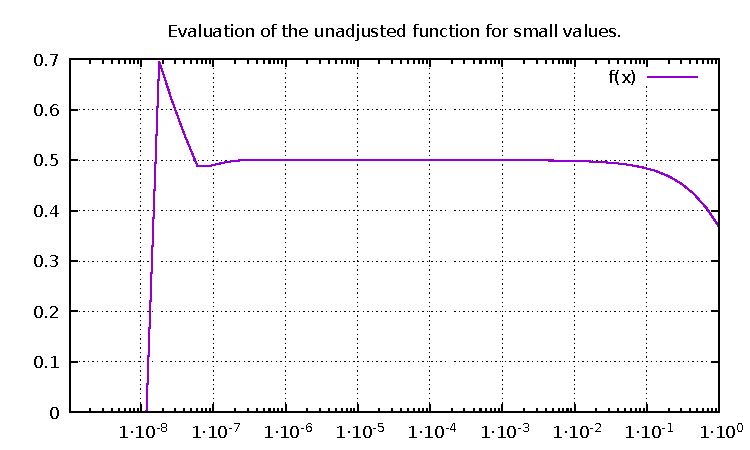
\includegraphics[width=0.8\textwidth]{../analysis/f.pdf}
    \caption{Evaluation of the function for small values.}
    \label{fig::f}
\end{figure}


\subsection{Explanation for the failure of the formula for small values}


\subsection{Adjustment for the calculation of the function.}

To get around the problem with the small values an if-statement can be
added to the execution of the function. This conditional case
will only be executed if the values of x are beneath the threshhold determined 
previously.\\
In order to get correct results for values beneath this threshhold
a different formular is needed. This can be done with the taylor
expansion of the function (1) which is given by:

\begin{align}
    f(x) = \sum_{n=0}^{\inf}\frac{(-x)^n}{(n+2)!}    
\end{align} 

Using the first three terms of this formular as an adustment to the function the overall 
results become reasonable. This is illustrated in figure \ref{fig::adjustedF}.

\begin{figure}[h]
    \centering
    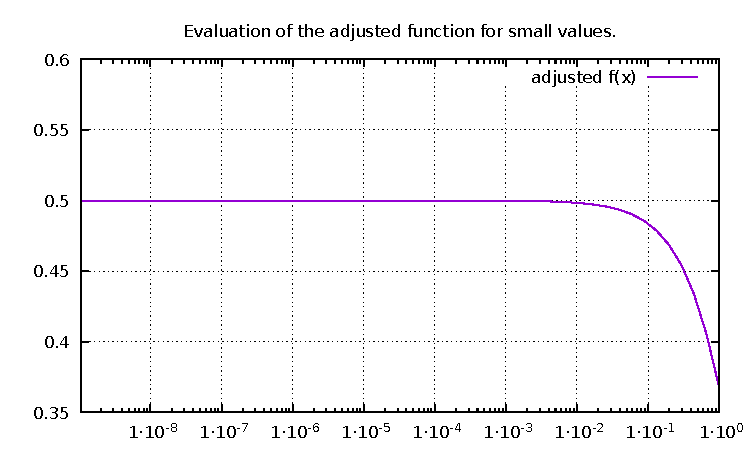
\includegraphics[width=0.8\textwidth]{../analysis/adjustedF.pdf}
    \caption{Evaluation of the adjusted function for small values.}
    \label{fig::adjustedF}
\end{figure}

\end{document}
